\chapter{Performance of our VO Pipline}
\label{performance}

\section{Effect of Bundle Adjustment}
- ref to fig of aligned trajectory w/ and w/o BA
- timing 
- discussion
- Bundle Adjustment decreases the maximum framerate by a factor x
- toAdjustOrNotToAdjust

\section{Error Analysis of Params}

In order to do a thorough optimization, a total of 15 parameters would have to varied simultaneously. 
This would lead to an intractable number of valid combinations. To curb the computational burden we proceeded to group the parameters into three main clusters:

\begin{itemize}
    \item Harris corner detection (harris\_kappa, harris\_patch\_size)
    \item candidate adding (candidate\_cap, candidate\_add, nonmaximum\_supression\_radius)
    \item repeated optimization with most sensitive parameters.
\end{itemize}

First, a sane parameter configuration was guessed for each cluster. Then, groups were fine tuned in a parallel simulation setup \coderef{simTaskScheduler.m}. Parameters were selected whenever a significant impact on accuracy (deviation from ground truth, see chapter \ref{simulation}) and robustness (successful completion of simulation challenge with varying other parameters) was detected.

\subsection{Harris Tuning}
From a qualitative observation of the trajectories, we could observe that features detected with a patch size of 9 and a kappa of 0.08 result in low tracking loss when applied on the provided data sets.

%warping = verwerfen
\subsection{Candidate Reinforcement Tuning (adding of candidates)} 
The goal of reinforcement tuning was to find a relation in between key point generation, warping and the overall pipeline performance. Tuning parameters were known to limit or boost key point generation or warping. A quantitative error analysis was performed for 4 parameters. The following impacts were measured:

\begin{itemize}
    \item Suppress\_existing\_matches strongly improves the algorithm stability.
    \item The candidate\_cap has negligible impact on the precision when above 500.
    \item Large variation was found in nonmaximum\_supression\_radius (selected for parameter tuning).
    \item Large variation was found in add\_candidate\_each\_frame (selected for parameter tuning).
\end{itemize}

\subsection{Significant Parameter Tuning}  
From empirical studies (trial and error) sensitive (high impact) parameters were identified and interesting ranges were selected for the final optimization. 
The parameters in table \ref{table:significant-param-tuning} were considered most relevant (as seen in the reinforcement tuning). 
As can be seen in figure \ref{fig:error_histogram}, the variance of the orientation error is too small to make a significant statement.
Due to this the location error was considered for the evaluation.
Optimal parameters were selected systematically by first evaluating the best 10 results (see figure \ref{fig:best10}).
Then, we cross verified the parameter tendency with the best 200 results to verify the trust-ability of the assumption. (see figure \ref{fig:best200}). The last step is to test the parameter robustness (see figure \ref{fig:exceptions}). 
Scale drift is a problem that cannot be solved with parameter tuning and must be addressed with BA.

\begin{table}[]
	\centering
	\caption{Significant parameter tuning: best three results. The maximum average location error was 23187, the minimal error 6664.9 and the median was 16059.0. }
	\label{table:significant-param-tuning}
	\begin{tabular}{lrrrr}
		\hline
		\textbf{Parameters}                &         \textbf{Range} & \textbf{Best} & \textbf{2nd Best} & \textbf{3rd Best} \\ \hline
		Average Error Score                &                        &          6664 &              6987 &              7207 \\ \hline\hline
		nonmaximum\_supression\_radius     &                10:2:16 &            12 &                10 &                10 \\ \hline
		add\_candidate\_each\_frame        &              50:50:200 &           150 &               200 &               200 \\ \hline
		triangulate\_max\_repr\_error      & [0.5, 1, 2, 5, 10, 20] &             5 &                 5 &                 5 \\ \hline
		critical\_kp                       &       [0, 20, 50, 100] &           100 &                 0 &                 0 \\ \hline
		tracker\_max\_bidirectional\_error &      [2.1, 5, 9999999] &             5 &               2,1 &                 5 \\ \hline
	\end{tabular}
\end{table}



\begin{figure}[htp]
	\centering
	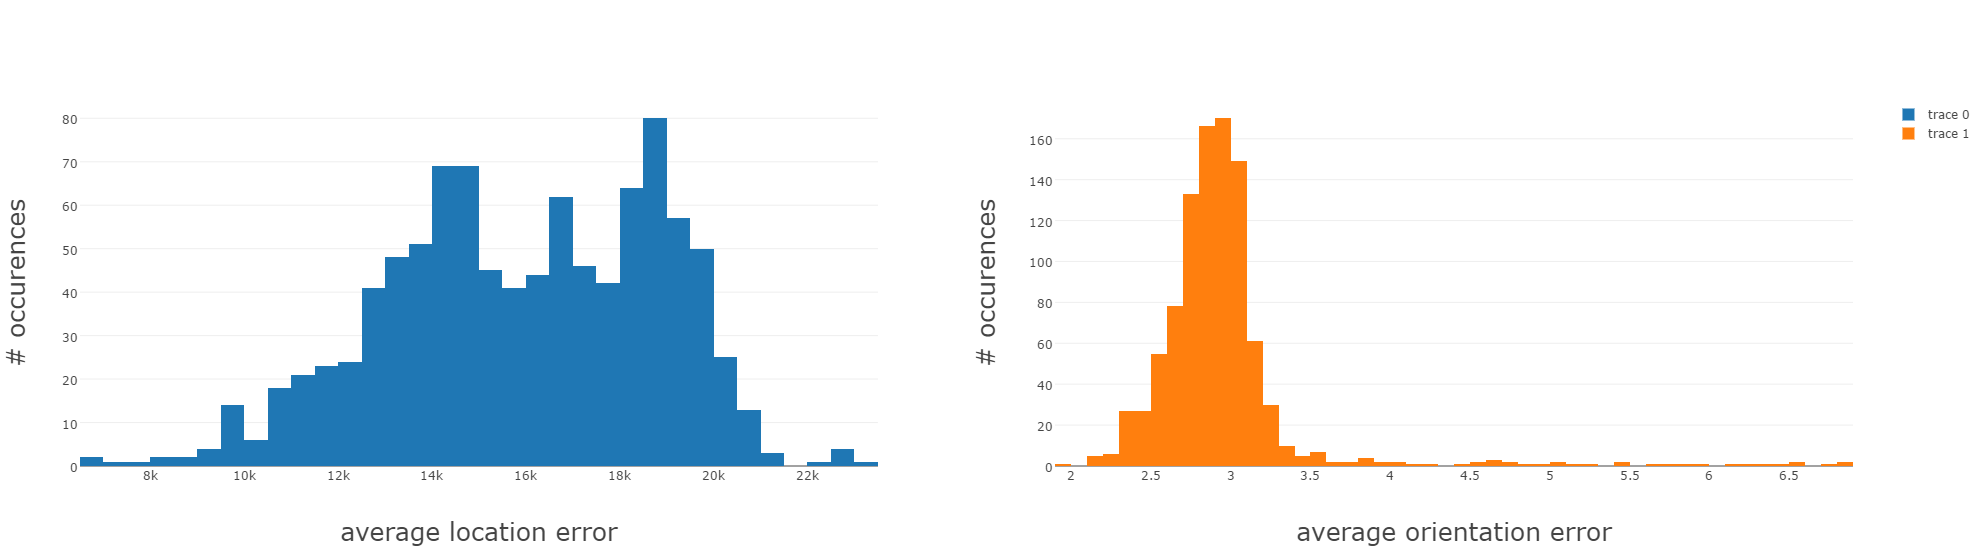
\includegraphics[width=1\textwidth]{figures/error_histogram}
	\caption{Distribution of the location error $LE$ and orientation error $OE$. An outlier (23.79) was removed from the orientation errors. 
		$OE_{min}: 1.97$, 
		$OE_{max}: 23.79$,
		$OE_{med}: 2.89$,
		$LE_{min}: 6664.9$,
		$LE_{max}: 23187.5$,
		$LE_{med}: 16059.0$}
	\label{fig:error_histogram}
\end{figure}


\begin{figure}[htp]
	\centering
	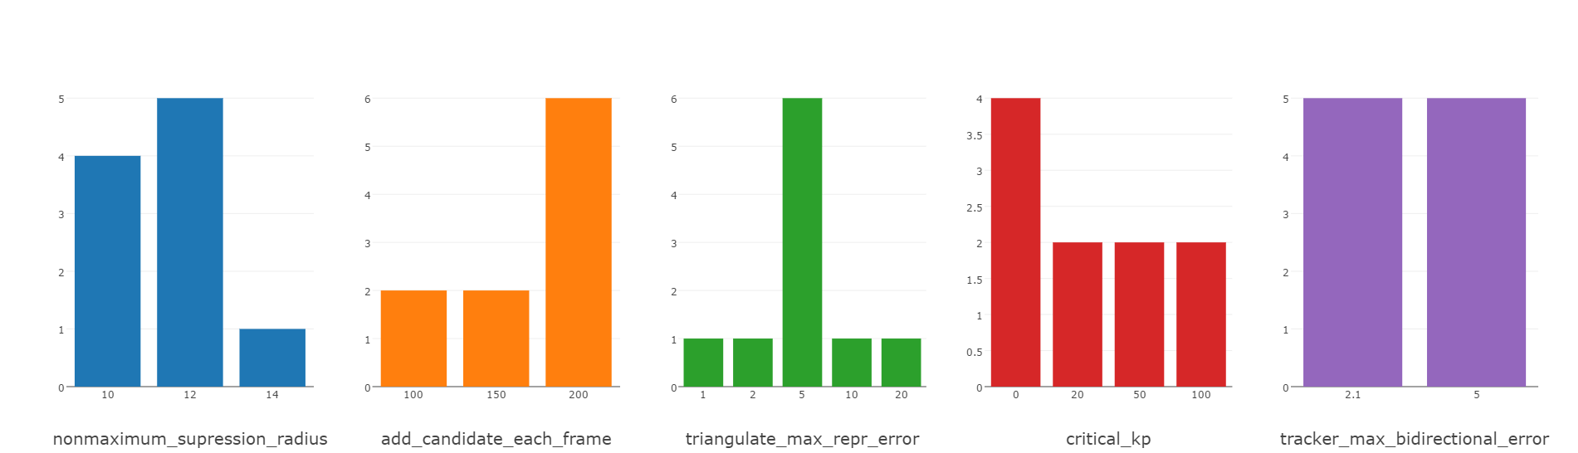
\includegraphics[width=1\textwidth]{figures/best10}
	\caption{Parameter distribution of the best 10 results  (15\% of the dynamic range).}
	\label{fig:best10}
\end{figure}



\begin{figure}[htp]
	\centering
	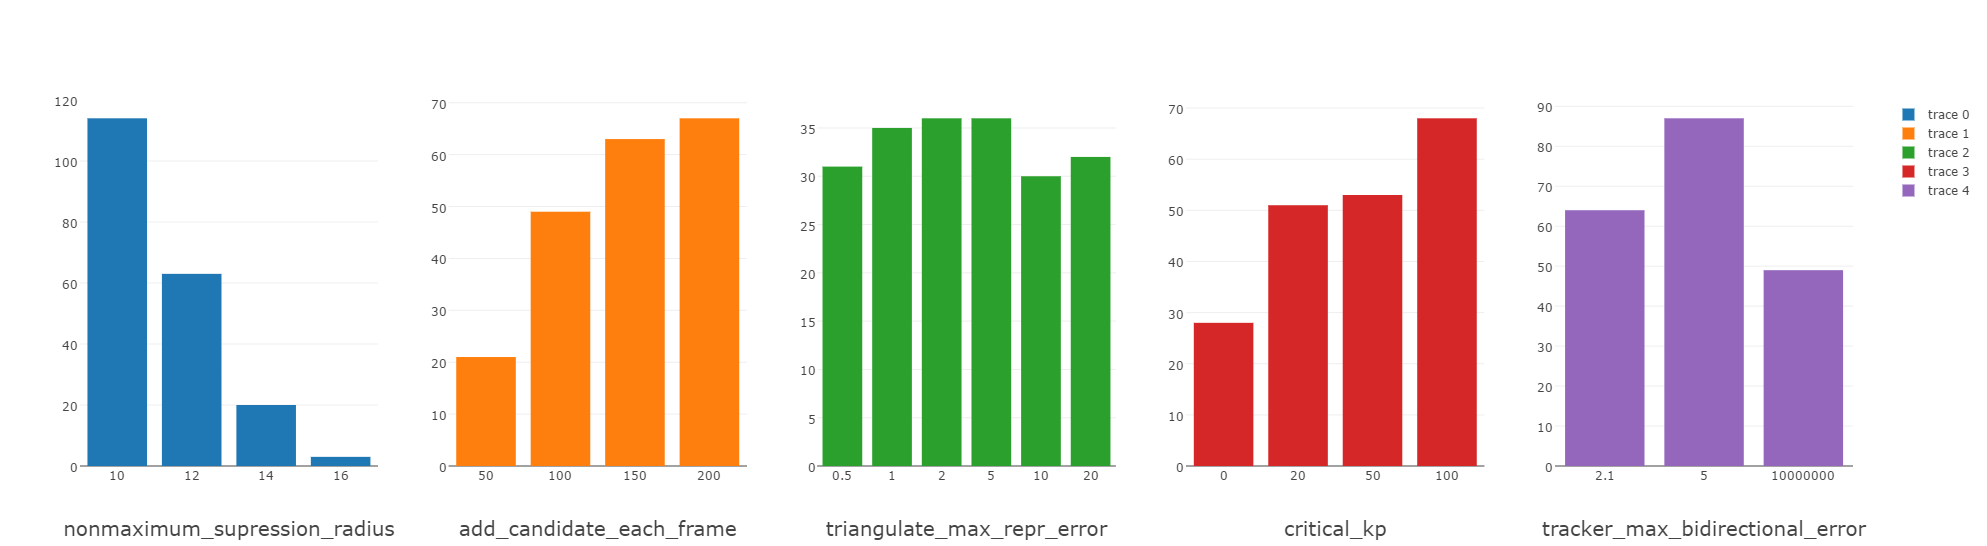
\includegraphics[width=1\textwidth]{figures/best200}
	\caption{Parameter distribution of the best 200 results  (40\% of the dynamic range).}
	\label{fig:best200}
\end{figure}



\begin{figure}[htp]
	\centering
	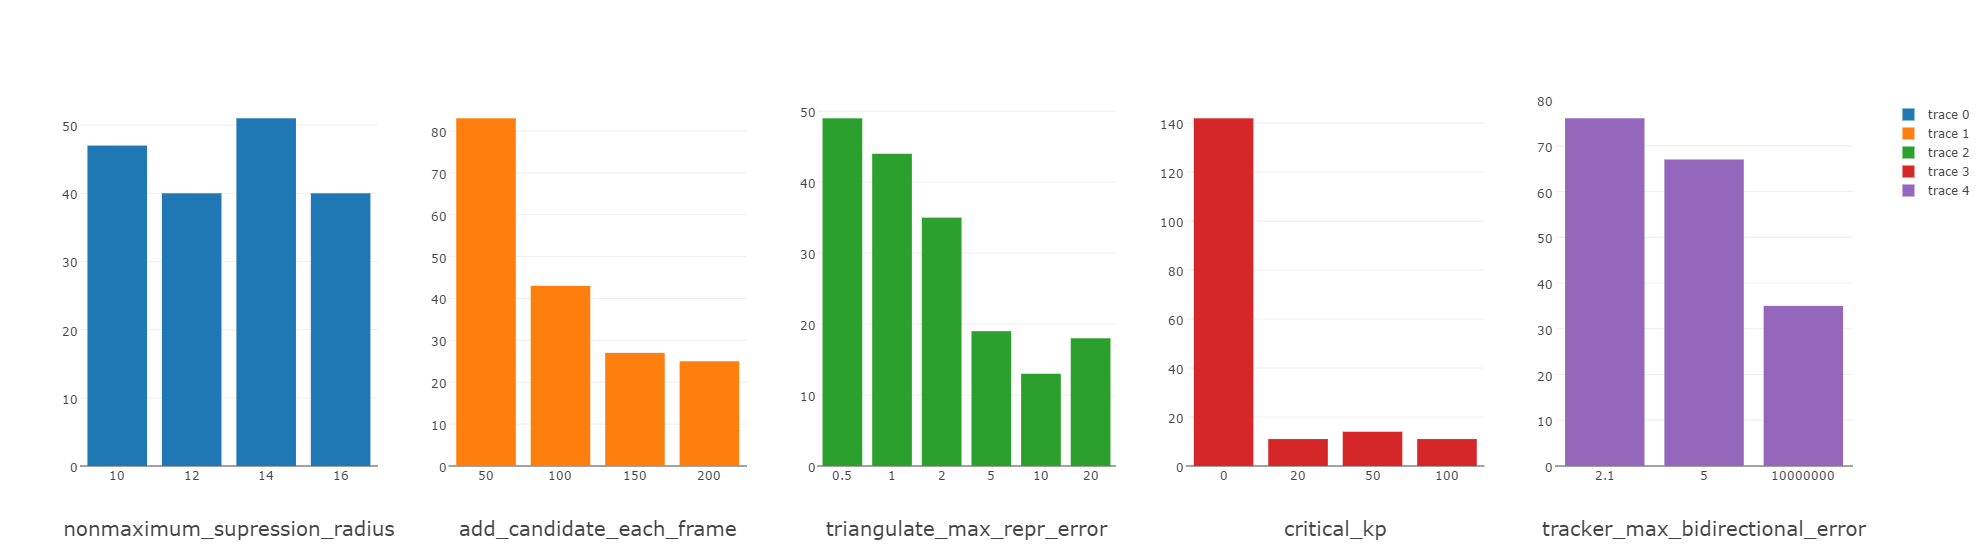
\includegraphics[width=1\textwidth]{figures/exceptions}
	\caption{Parameter distribution of all runs that terminated due to loss of key point tracking. }
	\label{fig:exceptions}
\end{figure}






